\documentclass[twoside]{book}

% Packages required by doxygen
\usepackage{fixltx2e}
\usepackage{calc}
\usepackage{doxygen}
\usepackage[export]{adjustbox} % also loads graphicx
\usepackage{graphicx}
\usepackage[utf8]{inputenc}
\usepackage{makeidx}
\usepackage{multicol}
\usepackage{multirow}
\PassOptionsToPackage{warn}{textcomp}
\usepackage{textcomp}
\usepackage[nointegrals]{wasysym}
\usepackage[table]{xcolor}

% Font selection
\usepackage[T1]{fontenc}
\usepackage[scaled=.90]{helvet}
\usepackage{courier}
\usepackage{amssymb}
\usepackage{sectsty}
\renewcommand{\familydefault}{\sfdefault}
\allsectionsfont{%
  \fontseries{bc}\selectfont%
  \color{darkgray}%
}
\renewcommand{\DoxyLabelFont}{%
  \fontseries{bc}\selectfont%
  \color{darkgray}%
}
\newcommand{\+}{\discretionary{\mbox{\scriptsize$\hookleftarrow$}}{}{}}

% Page & text layout
\usepackage{geometry}
\geometry{%
  a4paper,%
  top=2.5cm,%
  bottom=2.5cm,%
  left=2.5cm,%
  right=2.5cm%
}
\tolerance=750
\hfuzz=15pt
\hbadness=750
\setlength{\emergencystretch}{15pt}
\setlength{\parindent}{0cm}
\setlength{\parskip}{3ex plus 2ex minus 2ex}
\makeatletter
\renewcommand{\paragraph}{%
  \@startsection{paragraph}{4}{0ex}{-1.0ex}{1.0ex}{%
    \normalfont\normalsize\bfseries\SS@parafont%
  }%
}
\renewcommand{\subparagraph}{%
  \@startsection{subparagraph}{5}{0ex}{-1.0ex}{1.0ex}{%
    \normalfont\normalsize\bfseries\SS@subparafont%
  }%
}
\makeatother

% Headers & footers
\usepackage{fancyhdr}
\pagestyle{fancyplain}
\fancyhead[LE]{\fancyplain{}{\bfseries\thepage}}
\fancyhead[CE]{\fancyplain{}{}}
\fancyhead[RE]{\fancyplain{}{\bfseries\leftmark}}
\fancyhead[LO]{\fancyplain{}{\bfseries\rightmark}}
\fancyhead[CO]{\fancyplain{}{}}
\fancyhead[RO]{\fancyplain{}{\bfseries\thepage}}
\fancyfoot[LE]{\fancyplain{}{}}
\fancyfoot[CE]{\fancyplain{}{}}
\fancyfoot[RE]{\fancyplain{}{\bfseries\scriptsize Generated by Doxygen }}
\fancyfoot[LO]{\fancyplain{}{\bfseries\scriptsize Generated by Doxygen }}
\fancyfoot[CO]{\fancyplain{}{}}
\fancyfoot[RO]{\fancyplain{}{}}
\renewcommand{\footrulewidth}{0.4pt}
\renewcommand{\chaptermark}[1]{%
  \markboth{#1}{}%
}
\renewcommand{\sectionmark}[1]{%
  \markright{\thesection\ #1}%
}

% Indices & bibliography
\usepackage{natbib}
\usepackage[titles]{tocloft}
\setcounter{tocdepth}{3}
\setcounter{secnumdepth}{5}
\makeindex

% Hyperlinks (required, but should be loaded last)
\usepackage{ifpdf}
\ifpdf
  \usepackage[pdftex,pagebackref=true]{hyperref}
\else
  \usepackage[ps2pdf,pagebackref=true]{hyperref}
\fi
\hypersetup{%
  colorlinks=true,%
  linkcolor=blue,%
  citecolor=blue,%
  unicode%
}

% Custom commands
\newcommand{\clearemptydoublepage}{%
  \newpage{\pagestyle{empty}\cleardoublepage}%
}

\usepackage{caption}
\captionsetup{labelsep=space,justification=centering,font={bf},singlelinecheck=off,skip=4pt,position=top}

%===== C O N T E N T S =====

\begin{document}

% Titlepage & ToC
\hypersetup{pageanchor=false,
             bookmarksnumbered=true,
             pdfencoding=unicode
            }
\pagenumbering{roman}
\begin{titlepage}
\vspace*{7cm}
\begin{center}%
{\Large My Project }\\
\vspace*{1cm}
{\large Generated by Doxygen 1.8.11}\\
\end{center}
\end{titlepage}
\clearemptydoublepage
\tableofcontents
\clearemptydoublepage
\pagenumbering{arabic}
\hypersetup{pageanchor=true}

%--- Begin generated contents ---
\chapter{Hierarchical Index}
\section{Class Hierarchy}
This inheritance list is sorted roughly, but not completely, alphabetically\+:\begin{DoxyCompactList}
\item \contentsline{section}{g1\+:\+:gateway}{\pageref{structg1_1_1gateway}}{}
\item \contentsline{section}{g1\+:\+:package}{\pageref{structg1_1_1package}}{}
\begin{DoxyCompactList}
\item \contentsline{section}{g1\+:\+:controlled\+\_\+package}{\pageref{structg1_1_1controlled__package}}{}
\end{DoxyCompactList}
\item \contentsline{section}{g1\+:\+:package\+\_\+header}{\pageref{structg1_1_1package__header}}{}
\end{DoxyCompactList}

\chapter{Class Index}
\section{Class List}
Here are the classes, structs, unions and interfaces with brief descriptions\+:\begin{DoxyCompactList}
\item\contentsline{section}{\hyperlink{structg1_1_1package__block}{g1\+::package\+\_\+block} \\*Структура-\/описатель блока. Создается поверх пакета для упрощения работы с ним }{\pageref{structg1_1_1package__block}}{}
\item\contentsline{section}{\hyperlink{structg1_1_1package__header}{g1\+::package\+\_\+header} \\*Структура заголовок пакета }{\pageref{structg1_1_1package__header}}{}
\end{DoxyCompactList}

\chapter{File Index}
\section{File List}
Here is a list of all documented files with brief descriptions\+:\begin{DoxyCompactList}
\item\contentsline{section}{/home/mirmik/project/g1/g1/{\bfseries gateway.\+h} }{\pageref{gateway_8h}}{}
\item\contentsline{section}{/home/mirmik/project/g1/g1/{\bfseries indexes.\+h} }{\pageref{indexes_8h}}{}
\item\contentsline{section}{/home/mirmik/project/g1/g1/\hyperlink{packet_8h}{packet.\+h} \\*Всё, что касается работы с пакетом }{\pageref{packet_8h}}{}
\item\contentsline{section}{/home/mirmik/project/g1/g1/\hyperlink{tower_8h}{tower.\+h} \\*Tower file }{\pageref{tower_8h}}{}
\end{DoxyCompactList}

\chapter{Class Documentation}
\hypertarget{structg1_1_1controlled__package}{}\section{g1\+:\+:controlled\+\_\+package Struct Reference}
\label{structg1_1_1controlled__package}\index{g1\+::controlled\+\_\+package@{g1\+::controlled\+\_\+package}}


Добавляет к пакету некоторые контрольные поля. Нужен для поддержки качества обслуживания.  




{\ttfamily \#include $<$package.\+h$>$}



Inheritance diagram for g1\+:\+:controlled\+\_\+package\+:
\nopagebreak
\begin{figure}[H]
\begin{center}
\leavevmode
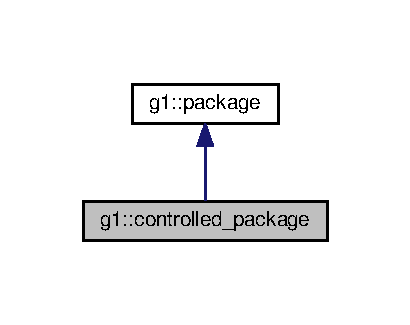
\includegraphics[width=197pt]{structg1_1_1controlled__package__inherit__graph}
\end{center}
\end{figure}


Collaboration diagram for g1\+:\+:controlled\+\_\+package\+:
\nopagebreak
\begin{figure}[H]
\begin{center}
\leavevmode
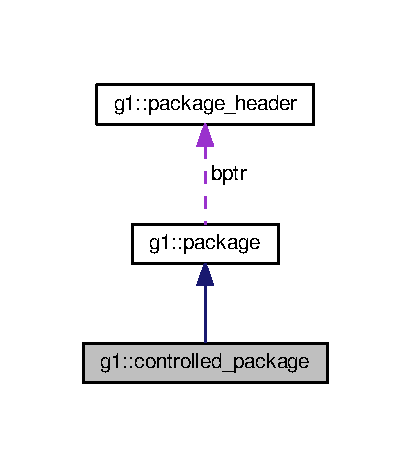
\includegraphics[width=197pt]{structg1_1_1controlled__package__coll__graph}
\end{center}
\end{figure}
\subsection*{Public Attributes}
\begin{DoxyCompactItemize}
\item 
dlist\+\_\+head \hyperlink{structg1_1_1controlled__package_aa9b5b38084ebcc0190d7fc05a62da482}{lnk}\hypertarget{structg1_1_1controlled__package_aa9b5b38084ebcc0190d7fc05a62da482}{}\label{structg1_1_1controlled__package_aa9b5b38084ebcc0190d7fc05a62da482}

\begin{DoxyCompactList}\small\item\em К списку хешированных пакетов. \end{DoxyCompactList}\item 
uint8\+\_\+t \hyperlink{structg1_1_1controlled__package_add10af1315e574984ceaed5fff274394}{resend\+\_\+count} = 0\hypertarget{structg1_1_1controlled__package_add10af1315e574984ceaed5fff274394}{}\label{structg1_1_1controlled__package_add10af1315e574984ceaed5fff274394}

\begin{DoxyCompactList}\small\item\em Счетчик попыток пересылки. \end{DoxyCompactList}\end{DoxyCompactItemize}
\subsection*{Additional Inherited Members}


\subsection{Detailed Description}
Добавляет к пакету некоторые контрольные поля. Нужен для поддержки качества обслуживания. 

The documentation for this struct was generated from the following file\+:\begin{DoxyCompactItemize}
\item 
/home/rfmeas/project/g1/g1/\hyperlink{package_8h}{package.\+h}\end{DoxyCompactItemize}

\hypertarget{structg1_1_1gateway}{}\section{g1\+:\+:gateway Struct Reference}
\label{structg1_1_1gateway}\index{g1\+::gateway@{g1\+::gateway}}


{\ttfamily \#include $<$gateway.\+h$>$}

\subsection*{Public Member Functions}
\begin{DoxyCompactItemize}
\item 
virtual void \hyperlink{structg1_1_1gateway_a5748219660a573356ab0e52f715eebbf}{send} (\hyperlink{structg1_1_1packet}{packet} $\ast$pack)=0
\begin{DoxyCompactList}\small\item\em Отправить пакет в целевой мир, согласно адресу стадии. \end{DoxyCompactList}\item 
int \hyperlink{structg1_1_1gateway_a8554ef0120b9fbb279087eb1d8c205dd}{receive\+\_\+handler} (void $\ast$buf, size\+\_\+t sz)
\begin{DoxyCompactList}\small\item\em Обработка пакета, пришедшего из другого мира. \end{DoxyCompactList}\end{DoxyCompactItemize}
\subsection*{Public Attributes}
\begin{DoxyCompactItemize}
\item 
dlist\+\_\+head \hyperlink{structg1_1_1gateway_a9b30f9f8c97681eb9b8ce01594200916}{lnk}\hypertarget{structg1_1_1gateway_a9b30f9f8c97681eb9b8ce01594200916}{}\label{structg1_1_1gateway_a9b30f9f8c97681eb9b8ce01594200916}

\begin{DoxyCompactList}\small\item\em встроенное поле списка. \end{DoxyCompactList}\item 
uint16\+\_\+t \hyperlink{structg1_1_1gateway_a9bc58cdaebf54c916deb87c4c44c0a59}{id}\hypertarget{structg1_1_1gateway_a9bc58cdaebf54c916deb87c4c44c0a59}{}\label{structg1_1_1gateway_a9bc58cdaebf54c916deb87c4c44c0a59}

\begin{DoxyCompactList}\small\item\em номер врат. \end{DoxyCompactList}\item 
gxx\+::dlist$<$ \hyperlink{structg1_1_1packet}{packet},\&\hyperlink{structg1_1_1packet_ad385dbb95d429aa9616059bd374b359b}{packet\+::lnk} $>$ \hyperlink{structg1_1_1gateway_af6c41db1fccaf674f06a8c0893238c1d}{packq}\hypertarget{structg1_1_1gateway_af6c41db1fccaf674f06a8c0893238c1d}{}\label{structg1_1_1gateway_af6c41db1fccaf674f06a8c0893238c1d}

\begin{DoxyCompactList}\small\item\em Очередь пакетов, ожидающих отправки. \end{DoxyCompactList}\end{DoxyCompactItemize}


\subsection{Detailed Description}
Абстрактный класс врат. Врата отвечают за пересылку пакетов между мирами. 

\subsection{Member Function Documentation}
\index{g1\+::gateway@{g1\+::gateway}!receive\+\_\+handler@{receive\+\_\+handler}}
\index{receive\+\_\+handler@{receive\+\_\+handler}!g1\+::gateway@{g1\+::gateway}}
\subsubsection[{\texorpdfstring{receive\+\_\+handler(void $\ast$buf, size\+\_\+t sz)}{receive_handler(void *buf, size_t sz)}}]{\setlength{\rightskip}{0pt plus 5cm}int g1\+::gateway\+::receive\+\_\+handler (
\begin{DoxyParamCaption}
\item[{void $\ast$}]{buf, }
\item[{size\+\_\+t}]{sz}
\end{DoxyParamCaption}
)}\hypertarget{structg1_1_1gateway_a8554ef0120b9fbb279087eb1d8c205dd}{}\label{structg1_1_1gateway_a8554ef0120b9fbb279087eb1d8c205dd}


Обработка пакета, пришедшего из другого мира. 

Здесь происходит реверт адреса и переправка в башню. \index{g1\+::gateway@{g1\+::gateway}!send@{send}}
\index{send@{send}!g1\+::gateway@{g1\+::gateway}}
\subsubsection[{\texorpdfstring{send(packet $\ast$pack)=0}{send(packet *pack)=0}}]{\setlength{\rightskip}{0pt plus 5cm}virtual void g1\+::gateway\+::send (
\begin{DoxyParamCaption}
\item[{{\bf packet} $\ast$}]{pack}
\end{DoxyParamCaption}
)\hspace{0.3cm}{\ttfamily [pure virtual]}}\hypertarget{structg1_1_1gateway_a5748219660a573356ab0e52f715eebbf}{}\label{structg1_1_1gateway_a5748219660a573356ab0e52f715eebbf}


Отправить пакет в целевой мир, согласно адресу стадии. 

Убить зверя. 
\begin{DoxyParams}{Parameters}
{\em pack} & Пересылаемый пакет \\
\hline
\end{DoxyParams}
\begin{DoxyReturn}{Returns}
Статус ошибки. 
\end{DoxyReturn}


The documentation for this struct was generated from the following file\+:\begin{DoxyCompactItemize}
\item 
/home/mirmik/project/g1/g1/gateway.\+h\end{DoxyCompactItemize}

\hypertarget{structg1_1_1package}{}\section{g1\+:\+:package Struct Reference}
\label{structg1_1_1package}\index{g1\+::package@{g1\+::package}}


Структура-\/описатель блока. Создается поверх пакета для упрощения работы с ним.  




{\ttfamily \#include $<$g1.\+h$>$}



Collaboration diagram for g1\+:\+:package\+:
\nopagebreak
\begin{figure}[H]
\begin{center}
\leavevmode
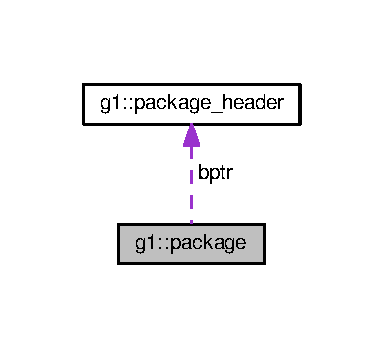
\includegraphics[width=184pt]{structg1_1_1package__coll__graph}
\end{center}
\end{figure}
\subsection*{Public Member Functions}
\begin{DoxyCompactItemize}
\item 
void \hyperlink{structg1_1_1package_a667ed03d442d2c9cfe28917c75525e4e}{revert\+\_\+stage} (uint8\+\_\+t size, void $\ast$addr)
\end{DoxyCompactItemize}
\subsection*{Public Attributes}
\begin{DoxyCompactItemize}
\item 
\hyperlink{structg1_1_1package__header}{package\+\_\+header} $\ast$ \hyperlink{structg1_1_1package_a1e75b5ccd00f3b8bd3c7958bc6d957e9}{bptr}\hypertarget{structg1_1_1package_a1e75b5ccd00f3b8bd3c7958bc6d957e9}{}\label{structg1_1_1package_a1e75b5ccd00f3b8bd3c7958bc6d957e9}

\begin{DoxyCompactList}\small\item\em Указатель на заголовок реферируемого блока \end{DoxyCompactList}\end{DoxyCompactItemize}


\subsection{Detailed Description}
Структура-\/описатель блока. Создается поверх пакета для упрощения работы с ним. 

\subsection{Member Function Documentation}
\index{g1\+::package@{g1\+::package}!revert\+\_\+stage@{revert\+\_\+stage}}
\index{revert\+\_\+stage@{revert\+\_\+stage}!g1\+::package@{g1\+::package}}
\subsubsection[{\texorpdfstring{revert\+\_\+stage(uint8\+\_\+t size, void $\ast$addr)}{revert_stage(uint8_t size, void *addr)}}]{\setlength{\rightskip}{0pt plus 5cm}void g1\+::package\+::revert\+\_\+stage (
\begin{DoxyParamCaption}
\item[{uint8\+\_\+t}]{size, }
\item[{void $\ast$}]{addr}
\end{DoxyParamCaption}
)}\hypertarget{structg1_1_1package_a667ed03d442d2c9cfe28917c75525e4e}{}\label{structg1_1_1package_a667ed03d442d2c9cfe28917c75525e4e}
Отметить в пакете прохождение врат. 

The documentation for this struct was generated from the following file\+:\begin{DoxyCompactItemize}
\item 
/home/rfmeas/project/g1/g1/\hyperlink{g1_8h}{g1.\+h}\end{DoxyCompactItemize}

\hypertarget{structg1_1_1package__header}{}\section{g1\+:\+:package\+\_\+header Struct Reference}
\label{structg1_1_1package__header}\index{g1\+::package\+\_\+header@{g1\+::package\+\_\+header}}


Структура заголовок пакета.  




{\ttfamily \#include $<$g1.\+h$>$}

\subsection*{Public Attributes}
\begin{DoxyCompactItemize}
\item 
uint8\+\_\+t \hyperlink{structg1_1_1package__header_a77aeda3b76d39b1067afd494c58873af}{type}\hypertarget{structg1_1_1package__header_a77aeda3b76d39b1067afd494c58873af}{}\label{structg1_1_1package__header_a77aeda3b76d39b1067afd494c58873af}

\begin{DoxyCompactList}\small\item\em Тип \end{DoxyCompactList}\item 
uint16\+\_\+t {\bfseries flen}\hypertarget{structg1_1_1package__header_a148b733fe97c06f0ded129f2a1d953c1}{}\label{structg1_1_1package__header_a148b733fe97c06f0ded129f2a1d953c1}

\item 
uint16\+\_\+t {\bfseries seqid}\hypertarget{structg1_1_1package__header_a8f706d30ff3d9154aff97827aa291af8}{}\label{structg1_1_1package__header_a8f706d30ff3d9154aff97827aa291af8}

\item 
uint8\+\_\+t {\bfseries alen}\hypertarget{structg1_1_1package__header_aca2dc89b824e81d9aaa99488aab21fe7}{}\label{structg1_1_1package__header_aca2dc89b824e81d9aaa99488aab21fe7}

\item 
uint8\+\_\+t {\bfseries stg}\hypertarget{structg1_1_1package__header_ade59c95e617ca8789a408c9aaa0ab088}{}\label{structg1_1_1package__header_ade59c95e617ca8789a408c9aaa0ab088}

\item 
\hyperlink{g1_8h_a157fb77f1b8142697dc1b88efaae6a0a}{QoS} {\bfseries qos}\hypertarget{structg1_1_1package__header_aea47ad75b2af7d91d1f460ff5887c751}{}\label{structg1_1_1package__header_aea47ad75b2af7d91d1f460ff5887c751}

\end{DoxyCompactItemize}


\subsection{Detailed Description}
Структура заголовок пакета. 

The documentation for this struct was generated from the following file\+:\begin{DoxyCompactItemize}
\item 
/home/rfmeas/project/g1/g1/\hyperlink{g1_8h}{g1.\+h}\end{DoxyCompactItemize}

\chapter{File Documentation}
\hypertarget{package_8h}{}\section{/home/mirmik/project/g1/g1/package.h File Reference}
\label{package_8h}\index{/home/mirmik/project/g1/g1/package.\+h@{/home/mirmik/project/g1/g1/package.\+h}}


Всё, что касается работы с пакетом.  


{\ttfamily \#include $<$cstdint$>$}\\*
Include dependency graph for package.\+h\+:\nopagebreak
\begin{figure}[H]
\begin{center}
\leavevmode
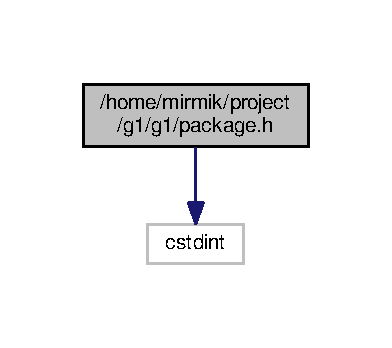
\includegraphics[width=188pt]{package_8h__incl}
\end{center}
\end{figure}
\subsection*{Classes}
\begin{DoxyCompactItemize}
\item 
struct \hyperlink{structg1_1_1package__header}{g1\+::package\+\_\+header}
\begin{DoxyCompactList}\small\item\em Структура заголовок пакета. \end{DoxyCompactList}\item 
struct \hyperlink{structg1_1_1package}{g1\+::package}
\begin{DoxyCompactList}\small\item\em Структура-\/описатель блока. Создается поверх пакета для упрощения работы с ним. \end{DoxyCompactList}\end{DoxyCompactItemize}
\subsection*{Enumerations}
\begin{DoxyCompactItemize}
\item 
enum \hyperlink{package_8h_a157fb77f1b8142697dc1b88efaae6a0a}{g1\+::\+QoS} \+: uint8\+\_\+t \{ \hyperlink{package_8h_a157fb77f1b8142697dc1b88efaae6a0aa3a08e2a74d22aa3fcb0ba7207d30814e}{g1\+::\+One}, 
\hyperlink{package_8h_a157fb77f1b8142697dc1b88efaae6a0aada9a952d5dc002634dc185c74cd9b460}{g1\+::\+Two}, 
\hyperlink{package_8h_a157fb77f1b8142697dc1b88efaae6a0aa7cb9b75182ee893ea264e4a3097068e7}{g1\+::\+Three}
 \}\begin{DoxyCompactList}\small\item\em Качество обслуживания. \end{DoxyCompactList}
\end{DoxyCompactItemize}


\subsection{Detailed Description}
Всё, что касается работы с пакетом. 



\subsection{Enumeration Type Documentation}
\index{package.\+h@{package.\+h}!QoS@{QoS}}
\index{QoS@{QoS}!package.\+h@{package.\+h}}
\subsubsection[{\texorpdfstring{QoS}{QoS}}]{\setlength{\rightskip}{0pt plus 5cm}enum {\bf g1\+::\+QoS} \+: uint8\+\_\+t}\hypertarget{package_8h_file_a157fb77f1b8142697dc1b88efaae6a0a}{}\label{package_8h_file_a157fb77f1b8142697dc1b88efaae6a0a}


Качество обслуживания. 

\begin{Desc}
\item[Enumerator]\par
\begin{description}
\index{One@{One}!package.\+h@{package.\+h}}\index{package.\+h@{package.\+h}!One@{One}}\item[{\em 
One\hypertarget{package_8h_a157fb77f1b8142697dc1b88efaae6a0aa3a08e2a74d22aa3fcb0ba7207d30814e}{}\label{package_8h_a157fb77f1b8142697dc1b88efaae6a0aa3a08e2a74d22aa3fcb0ba7207d30814e}
}]one \index{Two@{Two}!package.\+h@{package.\+h}}\index{package.\+h@{package.\+h}!Two@{Two}}\item[{\em 
Two\hypertarget{package_8h_a157fb77f1b8142697dc1b88efaae6a0aada9a952d5dc002634dc185c74cd9b460}{}\label{package_8h_a157fb77f1b8142697dc1b88efaae6a0aada9a952d5dc002634dc185c74cd9b460}
}]two \index{Three@{Three}!package.\+h@{package.\+h}}\index{package.\+h@{package.\+h}!Three@{Three}}\item[{\em 
Three\hypertarget{package_8h_a157fb77f1b8142697dc1b88efaae6a0aa7cb9b75182ee893ea264e4a3097068e7}{}\label{package_8h_a157fb77f1b8142697dc1b88efaae6a0aa7cb9b75182ee893ea264e4a3097068e7}
}]three \end{description}
\end{Desc}

\hypertarget{tower_8h}{}\section{/home/mirmik/project/g1/g1/tower.h File Reference}
\label{tower_8h}\index{/home/mirmik/project/g1/g1/tower.\+h@{/home/mirmik/project/g1/g1/tower.\+h}}


tower file  


\subsection*{Functions}
\begin{DoxyCompactItemize}
\item 
void \hyperlink{tower_8h_a7fbcb90d84ad4b1dcdd2c09eac9c539c}{g1\+::transport} (\hyperlink{structg1_1_1package}{g1\+::package} pack)\hypertarget{tower_8h_a7fbcb90d84ad4b1dcdd2c09eac9c539c}{}\label{tower_8h_a7fbcb90d84ad4b1dcdd2c09eac9c539c}

\begin{DoxyCompactList}\small\item\em Переместить пакет дальше по конвееру врат. \end{DoxyCompactList}\item 
void \hyperlink{tower_8h_a750f6bfd94ccc8b6f47fc4fa94dd13bf}{g1\+::registry\+\_\+gate} (const \hyperlink{structg1_1_1gateway}{g1\+::gateway} \&gate)\hypertarget{tower_8h_a750f6bfd94ccc8b6f47fc4fa94dd13bf}{}\label{tower_8h_a750f6bfd94ccc8b6f47fc4fa94dd13bf}

\begin{DoxyCompactList}\small\item\em Подключить врата к башне. \end{DoxyCompactList}\end{DoxyCompactItemize}
\subsection*{Variables}
\begin{DoxyCompactItemize}
\item 
dlist$<$ \hyperlink{structg1_1_1gateway}{g1\+::gateway},\&\hyperlink{structg1_1_1gateway_a9b30f9f8c97681eb9b8ce01594200916}{g1\+::gateway\+::lnk} $>$ \hyperlink{tower_8h_a93a375fa1e7f88aa016b460f659ee244}{g1\+::gateways}\hypertarget{tower_8h_a93a375fa1e7f88aa016b460f659ee244}{}\label{tower_8h_a93a375fa1e7f88aa016b460f659ee244}

\begin{DoxyCompactList}\small\item\em Врата \end{DoxyCompactList}\end{DoxyCompactItemize}


\subsection{Detailed Description}
tower file 


%--- End generated contents ---

% Index
\backmatter
\newpage
\phantomsection
\clearemptydoublepage
\addcontentsline{toc}{chapter}{Index}
\printindex

\end{document}
